\documentclass{article}
\usepackage[utf8]{inputenc}
\usepackage[spanish]{babel}
\usepackage{listings}
\usepackage{graphicx}
\graphicspath{ {images/} }
\usepackage{cite}

\begin{document}

\begin{titlepage}
    \begin{center}
        \vspace*{1cm}
            
        \Huge
        \textbf{Ejercicio Calistenia}
            
        \vspace{0.5cm}
        \LARGE
            
        \vspace{1.5cm}
            
        \textbf{Miguel Hernando Martin Matiz}
            
        \vfill
            
        \vspace{0.8cm}
            
        \Large
        Despartamento de Ingeniería Electrónica y Telecomunicaciones\\
        Universidad de Antioquia\\
        Medellín\\
        Marzo de 2021
            
    \end{center}
\end{titlepage}

\tableofcontents
\newpage
\section{Acerca del ejercicio Calistenia}\label{intro}
Con este ejercicio se pretende conocer las diferentes soluciones planteadas por 3 personas las cuales son generadas a partir de una descripción dada en un documento con instrucciones para llevar unos obejtos de una posición (estado A) a otra (estado B).

\section{Documentación del ejercicio} \label{contenido}

\vspace{0.3cm}
\textbf{Objetos utilizados}: 

\begin{itemize}
\item 2 tarjetas tipo documento del mismo tamaño.
\item 1 hoja de papel tipo carta o cuaderno (en blanco o rayada).
\end{itemize}
\vspace{0.3cm}
El ejercicio se desarrolla en dos estados con una posición dada en la descripción para los objetos, partiendo de un estado inicial (estado A) y el estado final (estado B).

\vspace{0.3cm}
\textbf{Estado A:}
\vspace{0.3cm}

Poner dos tarjetas juntas del mismo tamaño, pegadas por el lado que tiene el área más grande. Las tarjetas se ponen sobre una superficie horizontal plana. Encima de las tarjetas se pone la hoja de papel buscando que queden centradas con respecto a cada borde de la hoja.

\vspace{0.3cm}
\textbf{Estado B:}
\vspace{0.3cm}

Levantar la hoja de papel y ponerla en otro lado, también sobre una superficie horizontal plana.
Tomar las tarjetas con una sola mano y ponerlas en la mitad de la hoja, también usando una sola mano y la misma mano, de manera que las tarjetas queden apoyadas sobre uno de sus bordes más cortos en la hoja y formando una especie de pirámide. Luego, tratar de que las tarjetas se queden en equilibrio, se sostengan solas y puedan dejar de cogerlas. El estado final termina cuando las tarjetas en posición de pirámide se queden allí quietas sin tocarlas.

\newpage
\section{Estados esperados} \label{imagenes}

En la Figura (\ref{fig:stateA}) y Figura (\ref{fig:stateB}), se presentan las posiciones del estado A y del estado B que se espera obtener como solución propuesta por cada persona a la que se le entregó la descripción del ejercicio.

\begin{figure}[h]
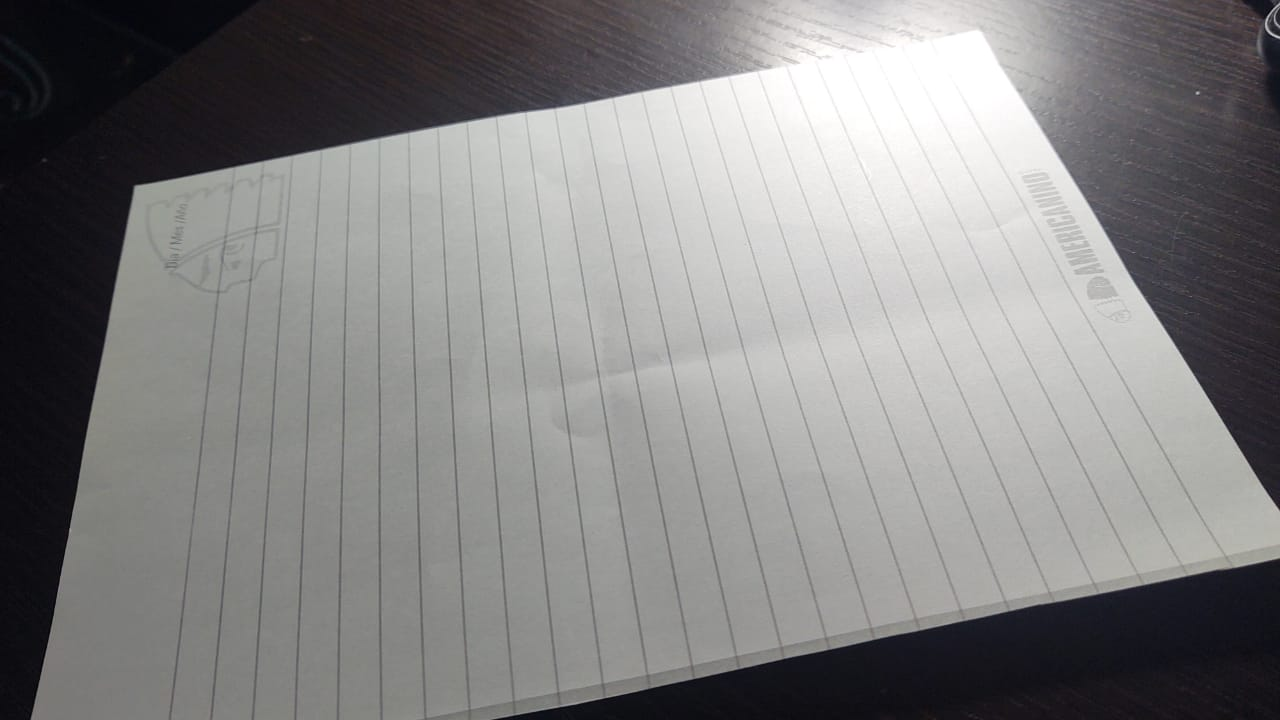
\includegraphics[width=10cm]{stateA.jpeg}
\centering
\caption{Estado A. Tarjetas debajo de la hoja.}
\label{fig:stateA}
\end{figure}

\begin{figure}[h]
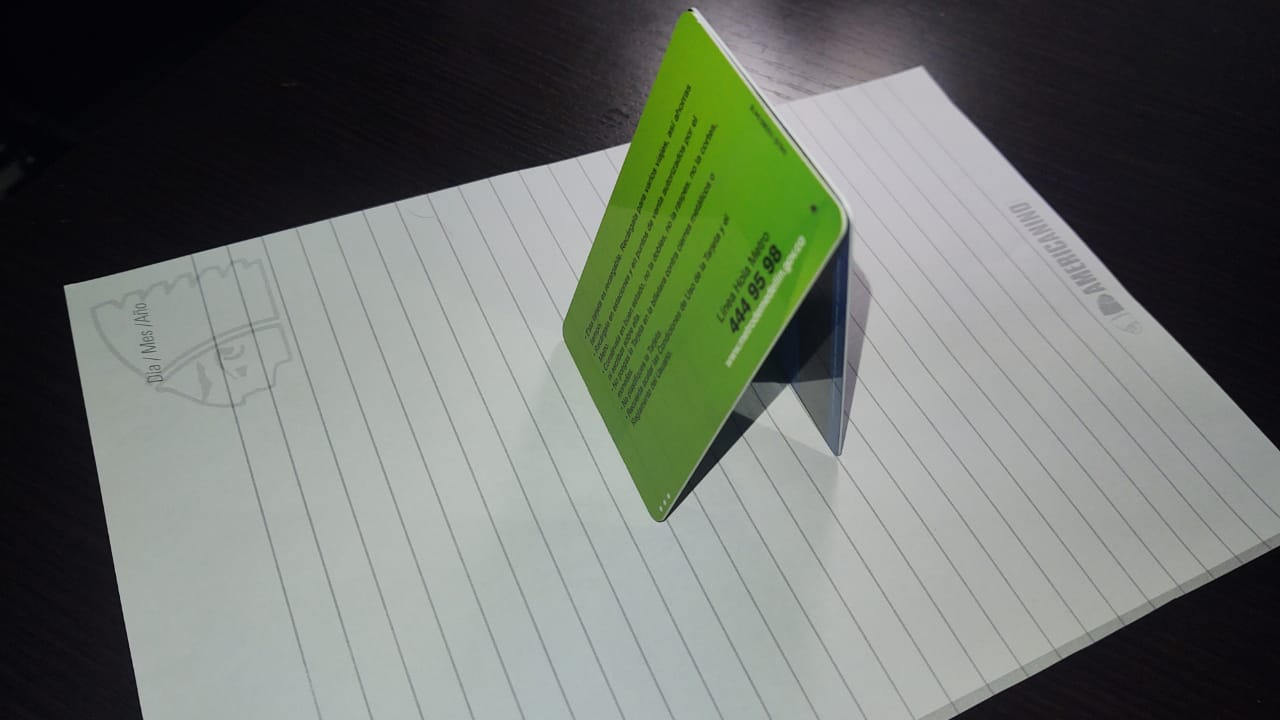
\includegraphics[width=10cm]{stateB.jpeg}
\centering
\caption{Estado B. Tarjetas en equilibrio.}
\label{fig:stateB}
\end{figure}

\end{document}